\documentclass[11pt]{article}

\usepackage{deauthor}
\usepackage{times,graphicx}

% user packages

\usepackage{url}
\usepackage{todonotes}
\usepackage{subcaption}
\usepackage{pifont}
\usepackage{newtxtext}
\usepackage{newtxmath}
\usepackage{newclude}
\usepackage{multirow}
\usepackage{hyperref}
\usepackage{CJK}
\usepackage{cite}
\usepackage{booktabs}
\usepackage{balance}
\newcommand{\xmark}{\ding{55}}
\newcommand{\cmark}{\ding{51}}

\renewcommand{\dblfloatpagefraction}{.9}

% unnecessary commands

\usepackage{paralist}
\newcommand{\entity}{\mathcal{E}}
\newcommand{\relation}{\mathcal{R}}
\newcommand{\lang}{\mathcal{L}}
\newcommand{\model}{\mathcal{M}}
\newcommand{\term}{\mathcal{T}}
\newcommand{\kgnew}{\mathcal{KG}}

\title{Implicit Sentiment Analysis of Chinese Texts \\ based on Contextual Information and Knowledge Enhancement}

\author{ Zhenghui Cao$^{\dagger}$
\hspace{2em}  Siqi Wang$^{\ddagger}$
\hspace{2em}  Haofen Wang$^{\ddagger}$ \thanks{*Corresponding author}
\hspace{2em}  Wenqiang Zhang$^{\dagger}$ \\
$^{\dagger}$ Fudan University, Shanghai, China \hspace{1em}
\texttt{\small\{caozh20,wqzhang\}@fudan.edu.cn}\\
$^{\ddagger}$ Tongji University, Shanghai, China \hspace{1em}
\texttt{\small \{siqi\_wang,nobot\}@tongji.edu.cn}}

\begin{document}

\maketitle

\section{Abstract}

The implicit sentiment analysis task makes the traditional explicit sentiment analysis methods no longer applicable due to the obscure and ambiguous expression of the sentiment text it focuses on and the lack of sentiment cue words containing obvious sentiment tendencies.
In this paper, we propose a sentiment analysis method incorporating contextual information and external common sense knowledge for implicit sentiment analysis.
We first propose a retrieval method to extract valid sentiment triples from a knowledge base and build an adaptive fusion of external common sense knowledge embedding layers to extend the semantic information of implicit sentiment expressions.
Multipolar orthogonal attention mechanism is then used to learn embedding representations for implicit sentiment expressions, and an attention layer that incorporates context is introduced to mine and combine valid information in the context.
Finally, the common sense knowledge information provided by the external knowledge base is fused with the contextual representation and the semantic information of the sentiment expression itself to achieve an effective extension of the implicit sentiment sentence representation and to perform sentiment label prediction.
Experimental results on the SMP2019-ECISA dataset show that the method outperforms existing state-of-the-art methods and can fully exploit contextual information and external common sense knowledge to effectively improve the analysis of implicit sentiment expressions.

\section{Introduction}

As one of the most popular research topics in the field of natural language processing, sentiment analysis tasks have been widely researched and applied in various fields such as academic research and product review mining, social opinion analysis, content-based recommendation, and so on.
People's experience and sentimental expression of objective things are often subjective and diverse, either by giving direct subjective statements of opinions, or by using facts or rhetorical hints to ideas, that is, by using sentences that do not contain obvious sentimental cues can also express a subjective sentiment. In connection with real life, people actually use a lot of implicit expressions to convey their feelings. There are examples as shown in the Fig~\ref{fig:Example}~.

\begin{figure}[h]
    \centering
    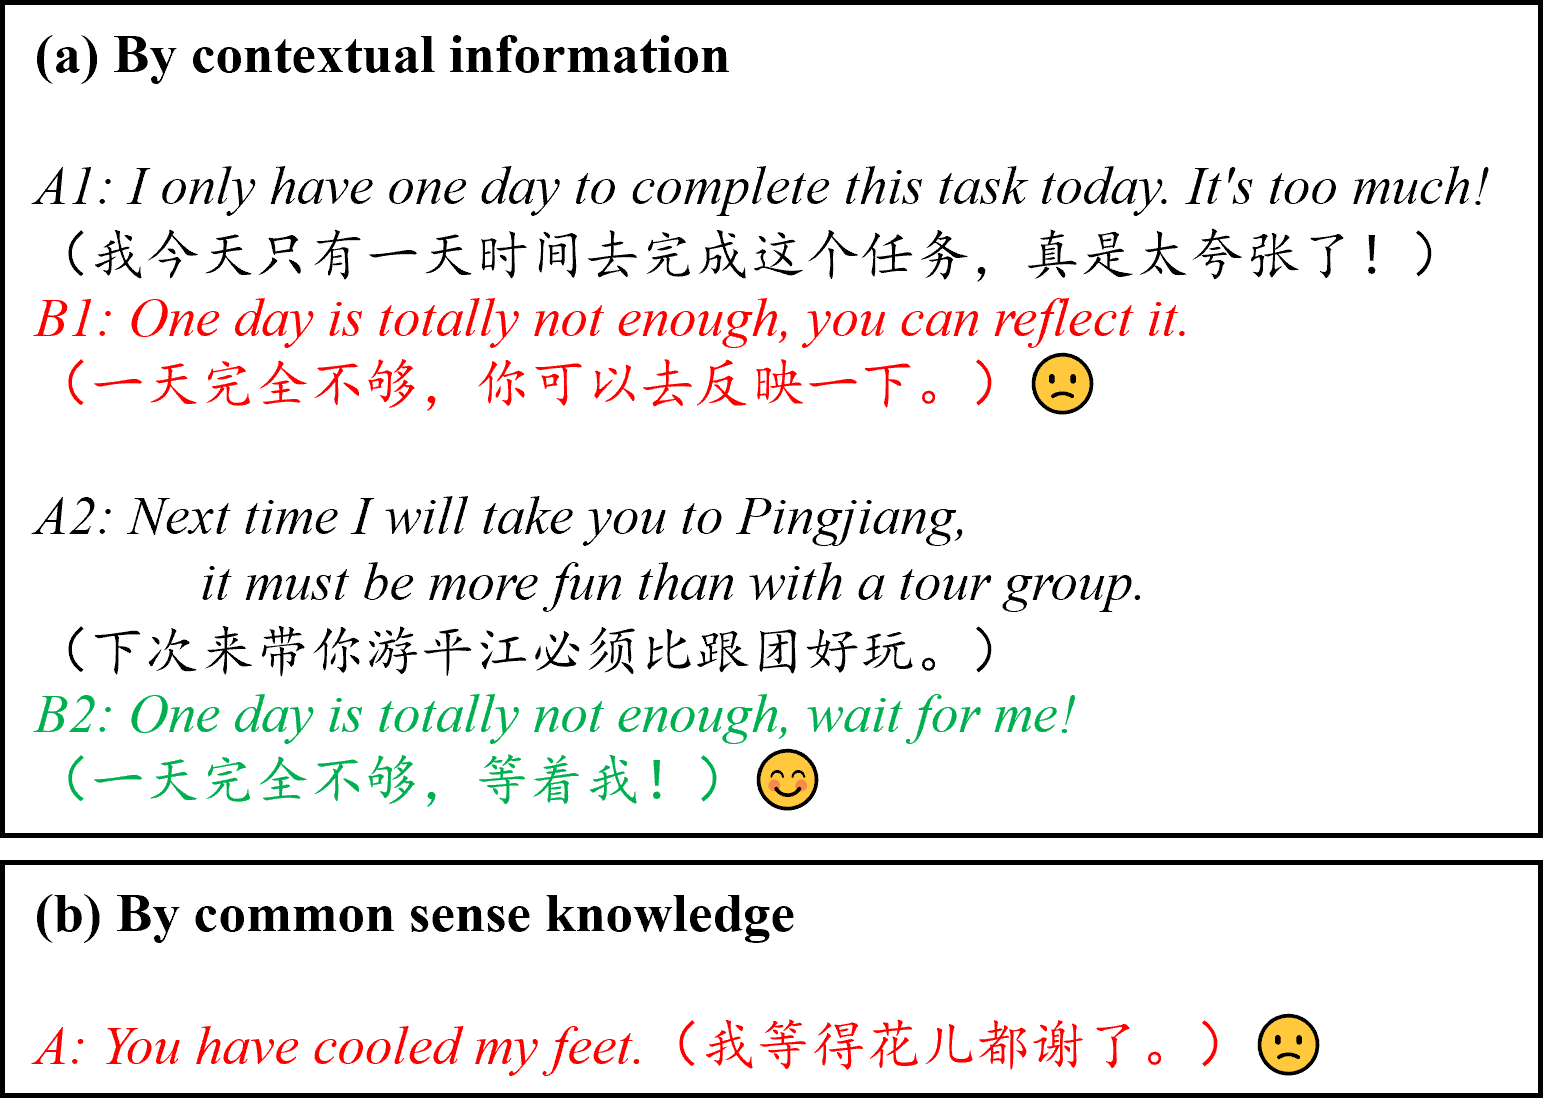
\includegraphics[width=0.5\linewidth]{submissions/knowledge-sentiment-analysis/2.png}
    \caption{Sentences with different contexts or based on external common sense knowledge can express different sentiments. Expressions carrying positive (smiling face) or negative (crying face) sentiments are highlighted in color. }
    \label{fig:Example}
\end{figure}

Both of the above examples do not contain obvious sentimental cues, but they invariably convey the speaker's sentimental disposition.
Sentiment expressed implicitly rather than using words with sentimental colors are called ``implicit sentiment"\cite{PanDongXing2020}.
For the task of text sentiment analysis in natural language processing, sentiment texts can be classified into explicit sentiment analysis and implicit sentiment analysis according to whether they contain obvious sentiment words in their expressions\cite{liu2020sentiment}.
Statistical analysis of related studies\cite{jian2016constitution,chen2016implicit,liao2019identification} shows that implicit sentiment sentences are more common in Chinese, accounting for about 20\% to 30\% of all sentences with sentiment tendencies.
Explicit sentiment sentences contain explicit sentiment vocabulary with strong semantic feature information, which can help sentiment analysis models accurately predict the sentiment tendency in sentences, and therefore many research results have emerged in the field of explicit sentiment analysis.
On the contrary, implicit sentiment expressions do not have such characteristics, and the expressions are more obscure. For the current task of Chinese implicit sentiment analysis, there are two main critical problems faced:


Chinese implicit sentiment analysis requires the introduction of contextual information. Example (a) is an instance of the same expression expressing different sentimental tendencies in different contexts. The speaker conveys two opposite sentimental tendencies, negative (B1) and positive (B2), through the similar emotional expression ``One day is totally not enough" according to the content received above. Thus, implicit sentiment analysis suffers from the problem that the sentiment expression itself does not provide enough information, and contextual information needs to be introduced.

Chinese implicit sentiment analysis lacks the support of external knowledge. Example (b) is a declarative sentence using metaphorical rhetoric. Although it does not contain any sentimental cues such as ``anxious", etc., it effectively conveys the sentiment that the speaker has been waiting for a long time and is somewhat dissatisfied. Therefore, combined with human understanding of implicit sentimental expression, it is necessary to introduce an understanding of external common sense knowledge to support the discernment of implicit sentimental tendencies.

In order to address typical problems in Chinese implicit sentiment analysis tasks like those two listed above, we propose a sentiment analysis method in this paper that integrates contextual information and external common sense knowledge for implicit sentiment analysis.

The main contributions of this paper can be summarized as follows:

\begin{enumerate}

\item We propose a retrieval method to extract valid sentiment triads from a knowledge base and build an adaptive fusion of external common sense knowledge embedding layers to extend the semantic information of implicit sentiment expressions. Such improvements significantly facilitate the mining of implicit sentiment expressions hidden in ambiguous language fragments without sentiment words as clues.

\item Multipolar orthogonal attention mechanism is used to learn embedding representations for implicit sentiment expressions, and an attention layer that incorporates context is introduced to mine and combine valid information in the context. This effectively retains the differences between attention representations and thus contributes to distinguishing subtle differences between sentiment polarities.

\item The common sense knowledge information provided by the external knowledge base is fused with the contextual representation and the semantic information of the sentiment expression itself to achieve an effective extension of the implicit sentiment sentence representation and to perform sentiment label prediction. The experimental results show that our model obtains more satisfactory performance than the baseline models.

\end{enumerate} 
\section{Related Work}


Research related to implicit sentiment analysis is not fully developed compared to the field of explicit sentiment analysis\cite{erik2017sentiment,liu2020sentiment}.
For implicit sentiment, it can be divided into factual implicit sentiment and rhetorical implicit sentiment.
Rhetorical implicit sentiment can be subdivided into metaphorical or simile, rhetorical question, and ironic \cite{liao2019identification}.
Early research on implicit sentiment analysis focused on the task of identifying metaphors \cite{LiaoJian2018}, and as early as last century, Wilks et al. summarized metaphor, a common linguistic phenomenon, into a series of linguistic rules from the traditional cognitive and linguistic perspectives, through which metaphorical expressions and contexts, with the connections between them, are expressed.
Building on this theory, Mason et al. \cite{mason2004cormet} proposed a CorMet mapping of ``source domain-target domain" that can be identified by a specific domain, based on the linguistic feature that words can express different meanings in different domains. The CorMet model, which identifies between specific domains, was proposed.
Later, Lakoff \cite {J2008LakoffGeorge} studied the process of metaphorical expression in depth and defined it as a conceptual mapping from the source domain to the target domain in terms of cognition, common sense, etc.
In an earlier period, sentiment lexicon based methods played an important role in the field of sentiment analysis, but for implicit sentiment, the method could not be used directly for simple matching due to the lack of obvious sentiment words in the text variety.
Shutova et al.\cite{shutova2013statistical} addressed this problem to some extent by using clustering to obtain the abstract metaphors embedded in words; based on this work, the researchers went further to study the distribution of metaphorical concepts by combining weakly supervised and unsupervised approaches \cite{shutova2017multilingual}, and after experimentally testing several hierarchical clustering methods under specific constraints, a metaphorical pattern recognition algorithm was proposed, which achieved good results on a multilingual test set.
Zhang et al.\cite{zhang2011identifying} used sufficient collation and induction of sentiment texts to find that some phrases and special collocations, although without obvious sentiment cues, can implicitly express some implicit sentiment tendencies when they are expressed in sentences through metaphor or irony, and proposed a method to identify nouns with implicit sentiment domain features.
Balahur et al.\cite{balahur2011detecting}, on the other hand, focused on identifying the emotional tendency of the target with the help of contexts that do not contain emotion words, proposed an implicit sentiment analysis method based on common sense knowledge, and constructed an EmotiNet common sense knowledge base with relevant sentiment concepts; in subsequent work \cite{ balahur2012detecting}, the authors continued to improve their modeling method based on this common sense knowledge base and found that the sentiment of the target sentence could be discriminated from the context where all sentiments were implicitly expressed, and the experimental results showed that the method could effectively improve the effect of sentiment analysis.
Zhao et al.\cite{zhao2012collocation} took an alternative approach by introducing pseudo-contextual information into implicit sentiment analysis, and obtained the best results at that time in comparison experiments.
Tong et al. \cite{tong2013can} developed a theory-based discriminant system to analyze the relevance of ambiguous expressions to influence the euphemism of implicit affective utterances.
As deep learning methods are widely used in the field of sentiment analysis, many scholars have also started to use deep learning for implicit sentiment analysis tasks. Pulkit et al.\cite{mehndiratta2017detection} investigated recognition algorithms oriented to sarcastic expressions by using deep learning models. Qian et al.\cite{qian2018hierarchical} applied the idea of hierarchical classification to the task of identifying hate speech, and the method can effectively classify thirteen classes of hate speech categories.


In China, more and more scholars have started to focus on research targeting Chinese implicit sentiment analysis tasks in recent years.
Liao et al.\cite{liao2017freerl} first deconstructed the target text using syntactic analysis methods and proposed a representation learning framework based on tree convolution; immediately afterwards, the researchers in their paper \cite{LiaoJian2018,liao2019identification} provided a review of the work on Chinese implicit sentiment analysis, focusing on the characteristics of factual implicit sentiment; and based on word-level sentiment goals, sentence-level implicit sentiment expressions, and chapter-level contextual explicit sentiment tendencies, a multi-level semantic fusion representation learning approach was proposed for language modeling of factual implicit sentiment on two manually labeled factual implicit sentiment datasets. Experiments were conducted to verify that contextual information plays an important role in implicit sentiment recognition.
Wei et al. \cite{wei2020BiLSTM} proposed a multi-polar orthogonal attention model MPOA by comparing the differences between affective tendency features in social media texts, which also introduced a BERT pre-trained language model to represent the texts, and the experimental results showed that the model can effectively bridge the differences between words and affective tendency polarity corresponding to attention.
Zhao et al.\cite {ZhaoRongMei2020} proposed a hybrid neural network model based on CNN-BiLSTM-Attention, which extracts text features by CNN, obtains contextual information by Bi-LSTM. In addition, the model enables the extraction of semantic and structural features from the word and sentence levels respectively,  and highlights emotional information features that contribute more to emotional expressions by using the attention mechanism, and this hybrid model has improved the effectiveness of Chinese emotional utterance analysis.
Zuo et al. \cite{zuo2020context} proposed a context-specific heterogeneous graph convolution model (CsHGCN) , which introduces the idea of heterogeneous graphs into implicit sentiment analysis tasks and builds a contextual representation framework through graph convolutional neural networks, with improved results compared to network approaches such as tree graph convolution and tree long and short-term memory networks.
Yang et al. \cite {YangShanLiang2021} proposed an implicit sentiment analysis model based on graph attention neural network, by constructing a heterogeneous graph of text and word correspondences, aggregating semantic information using graph convolutional networks, and calculating the contribution of words with to the sentiment expression of the text using an attention mechanism, thus allowing the model to focus on words that are more important for sentiment polarity.
Chen et al.\cite {ChenQiuChang2022} proposed a parallel hybrid model of bidirectional long-short time neural network and context-aware tree recurrent neural network (CA-TRNN) for the problem of inaccurate feature information extraction in Chinese implicit sentiment analysis and gradient explosion or gradient disappearance for chapter-level text information extraction by existing serialization models, which effectively improved the accuracy of classification results with small time cost and better application capability.
In addition to digging deeper into the semantic information in Chinese implicit sentiment texts, the recognition of implicit sentiment usually requires the introduction of external sentiment features and sentiment knowledge.
Wang et al. \cite{wang2020chinese} fused three levels of semantic information in sentiment expressions, and proposed a method based on hierarchical knowledge enhancement to alleviate the problem of ``weak features" in Chinese implicit sentiment expressions, while introducing a multi-pooling approach to model the ``multiple confusion weak features" problem. The accuracy of the model has been effectively improved, and the F1 score is 5.9\% higher than the previous best model.

From the above review of existing research, it is clear that, in contrast to the task of explicit sentiment analysis, research on implicit sentiment analysis is still immature, remains in the exploratory stage and faces a large number of problems and challenges.

\section{Methodology}

\subsection{Problem Setup}

The definition of implicit sentiment in different research work \cite{PanDongXing2020,samuel2022direct,wang2020chinese} are slightly different. This paper integrates the expressions of the definitions, and defines implicit sentiment as: ``a fragment of language that does not directly contain obvious sentiment cues but expresses subjective sentiment", where ``fragment of language" includes words, phrases and sentences, and does not include a paragraph composed of several sentences. On this basis, this paper defines implicit sentiment analysis task as the task of ``sentiment analysis of Chinese implicit sentiment utterances that do not contain obvious sentiment words", and further abstracts it into a triple classification task, which classifies the possible sentiment tendencies of the sentences to be analyzed into `Positive', `Neutral', `Negative'.

The implicit sentiment analysis task is defined formally as follows: for any implicit sentiment sentence $ s = \{w_1,w_2,\dots,w_N\}$ and its context input to the model, output the model's prediction $P_t$ of sentence $s$ , and the Eq.~\ref{formula:classification-definition}~ defines the Chinese implicit sentiment sentence classification task.

\begin{equation}
    f(s) \rightarrow P_t=\left\{p_{t_0}, p_{t_1}, p_{t_2}\right\}\label{formula:classification-definition}
\end{equation}

where $N$ is the number of words contained in a given sentiment sentence, $w_n$ is the $n$th word in the sentence, $ n \in N $; $p_t$ is the probability that the implicit sentiment sentence $s$ belongs to a category, $p_{t_0}$ denotes the probability that the implicit sentiment sentence is neutral, $p_{t_1}$ denotes the probability that the implicit sentiment sentence is positive, $p_{t_2 }$ denotes the probability that the implicit sentiment sentence is negative.

\subsection{Knowledge Graph And Knowledge Retrieval}

Due to the lack of explicit sentiment words in implicit sentiment sentences, continuing to dig deeper into the semantic information latent in the text itself does not provide more adequate sentiment clues.
At this point, it is possible to associate the process of solving the problem with the human brain, which is to draw on rich external background knowledge.
Specifically, additional knowledge information can be introduced from the existing common sense knowledge graphs as sentiment cues for implicit sentiment analysis.

ConceptNet \footnote{https://conceptnet.io/} is a comprehensive commonsense knowledge graph, which is essentially a large semantic network describing concepts such as words and phrases that people use and the commonsense relationships between them, covering spatial, physical, social, temporal, and psychological aspects of everyday life.
ATOMIC \cite{sap2019atomic} is an event-centric knowledge graph. Recently, based on ATOMIC, Li et al. \cite{li2022c3kg} proposed a Chinese Commonsense Conversation Knowledge Graph (C3KG), which incorporates both social commonsense knowledge and dialog flow information, and is an important complement to Chinese common sense knowledge sources.

However, it is inefficient and unwise to retrieve sentiment knowledge triples directly in these huge knowledge bases which are oriented to almost all domains. Therefore, in this paper, a three-step triple extraction method is designed to extract valuable knowledge triples for the target implicit sentiment sentences.


\paragraph{Knowledge triples extraction based on rules}

The latest ConceptNet 5.5 includes a total of 34 different kinds of relations, and C3KG is divided into four main relationship patterns. The number of knowledge triples varies greatly across relationship types.
After analyzing the knowledge triples in the Chinese part of ConceptNet5, we found that the top 5 types of relationships account for more than 60\% of all relationships, including ``Synonym", ``RelatedTo", ``Causes", ``ExternalURL", and ``MotivatedByGoal''.
By observing the specific triple examples in ConceptNet5, it was obtained that the relations with the highest number of relations ``Synonym", ``RelatedTo" and others such as ``AtLocation'' have almost the same semantics between their corresponding head entity and tail entity or do not effectively provide additional sentiment cues, which leads to such relations being useless for sentiment analysis tasks. Instead, the model performance is greatly degraded by the large number of irrelevant knowledge retrieval processes and the introduction of redundant knowledge.
Similarly, for C3KG, it is observed that ``Emotion Cause Flow'', among the four relational models, has the greatest potential for implicit sentiment analysis tasks, while the other three relational models, ``emotion Intention Flow'', ``event flow'', and ``concept flow'', can only extend semantic information at the factual level, but do not introduce sentiment cues well.
Therefore, for the knowledge triple $t_k = (h, r, t) \in T$ (where $h$ and $t$ represent the head entity and tail entity, respectively, and $r$ denotes the relationship between two entities), the knowledge triples with these relationship types are firstly eliminated from the common knowledge base, which means only the triples with $ r \in R $ are retained, and $R$ denotes the set of valid relationships only after filtering.

Furthermore, in order to be able to introduce additional sentiment cues from the external knowledge graph efficiently, it is agreed that only one of the two, head entity $h$ and tail entity $t$, exists in the target implicit sentiment sentence $s \in C$.
With the above two rule constraints, it is possible to filter out those knowledge triples that introduce knowledge into the target implicit sentiment sentence.

\paragraph{Knowledge triples extraction based on sentiment dictionary matching}


After the rule-based knowledge triples extraction, in order to further extract the knowledge triples valuable for the implicit sentiment analysis task from the knowledge graph, explicit sentiment clues need to be introduced.
For the knowledge triple $t_k = (h, r, t) \in T$, $ h \in s $ or $ t \in s $, the entity not in the target implicit sentiment sentence is matched using the sentiment dictionary $d$, which is the concatenation of the three mainstream Chinese sentiment dictionaries. Knowledge triples without explicit sentiment cue words were subsequently eliminated.
After such matching and filtering, those sentiment knowledge triples with only one entity as an explicit sentiment word were selected to ensure that additional sentiment information could be introduced into the target implicit sentiment expression sentences.

\paragraph{Knowledge triples extraction based on event matching}

The sentiment knowledge triplets filtered by the above two filtering methods match the content of the target sentence at the character level. In order to be able to draw more fully on the relationship between events and sentiments embedded in the knowledge base, it is also necessary to extract sentiment events in the target sentences.

Sentiment expressions contain many colloquial expressions and complex sentence structures. In order to effectively extract sentiment events from the target implicit sentiment sentences, we adopt the same method for event extraction as that worked in the literature, and achieve effective extraction of sentiment events from the target implicit sentiment sentences through the methods and steps of Pre-processing, Verb-driven, Adjective-driven, and Recursive Applying.
For example, for the implicit sentiment expression ``Probably got a cold and stay up late, it is still some pain'', the sentiment event ``somebody gets cold'' can be extracted, which corresponds to the C3KG and can be associated to the sentiment triple $(personX\ gets\ cold, xAttr, Uncomfortable)$, and ``Uncomfortable'' is a negative sentiment tendency in the sentiment dictionary, thus introducing explicit sentiment cues.

Finally, since ConceptNet and C3KG are multilingual general knowledge base, although it contains some knowledge triples in Chinese, it is still more based on entity relationship pairs in English or other languages. For this reason, the knowledge in those knowledge bases are translated into Chinese as well as aligned and merged with the Chinese part through online translation. The merged knowledge graph is finally used as the main source of external knowledge in this paper.

\subsection{Sentiment Analysis Incorporating Contextual Information And External Common Sense Knowledge}

This method adaptively fuses knowledge from external common sense knowledge graphs by designing knowledge retrieval mechanisms in this paper in the process of learning textual representations.
By doing so, a process similar to that of the human brain in understanding implicit emotional expressions is simulated, i.e., drawing on one's own experience or common sense to distinguish sentiment tendencies, allowing the model to achieve a deeper understanding of the text beyond the literal semantic information.

The above model network framework diagram is shown in Fig~\ref{fig:framework-of-the-model}~. The model consists of four layers: input layer, adaptive knowledge fusion layer, multipolar attention layer fusing contextual contexts, and output layer. The structure of each layer is described in detail in the following.

\begin{figure}[h]
    \centering
    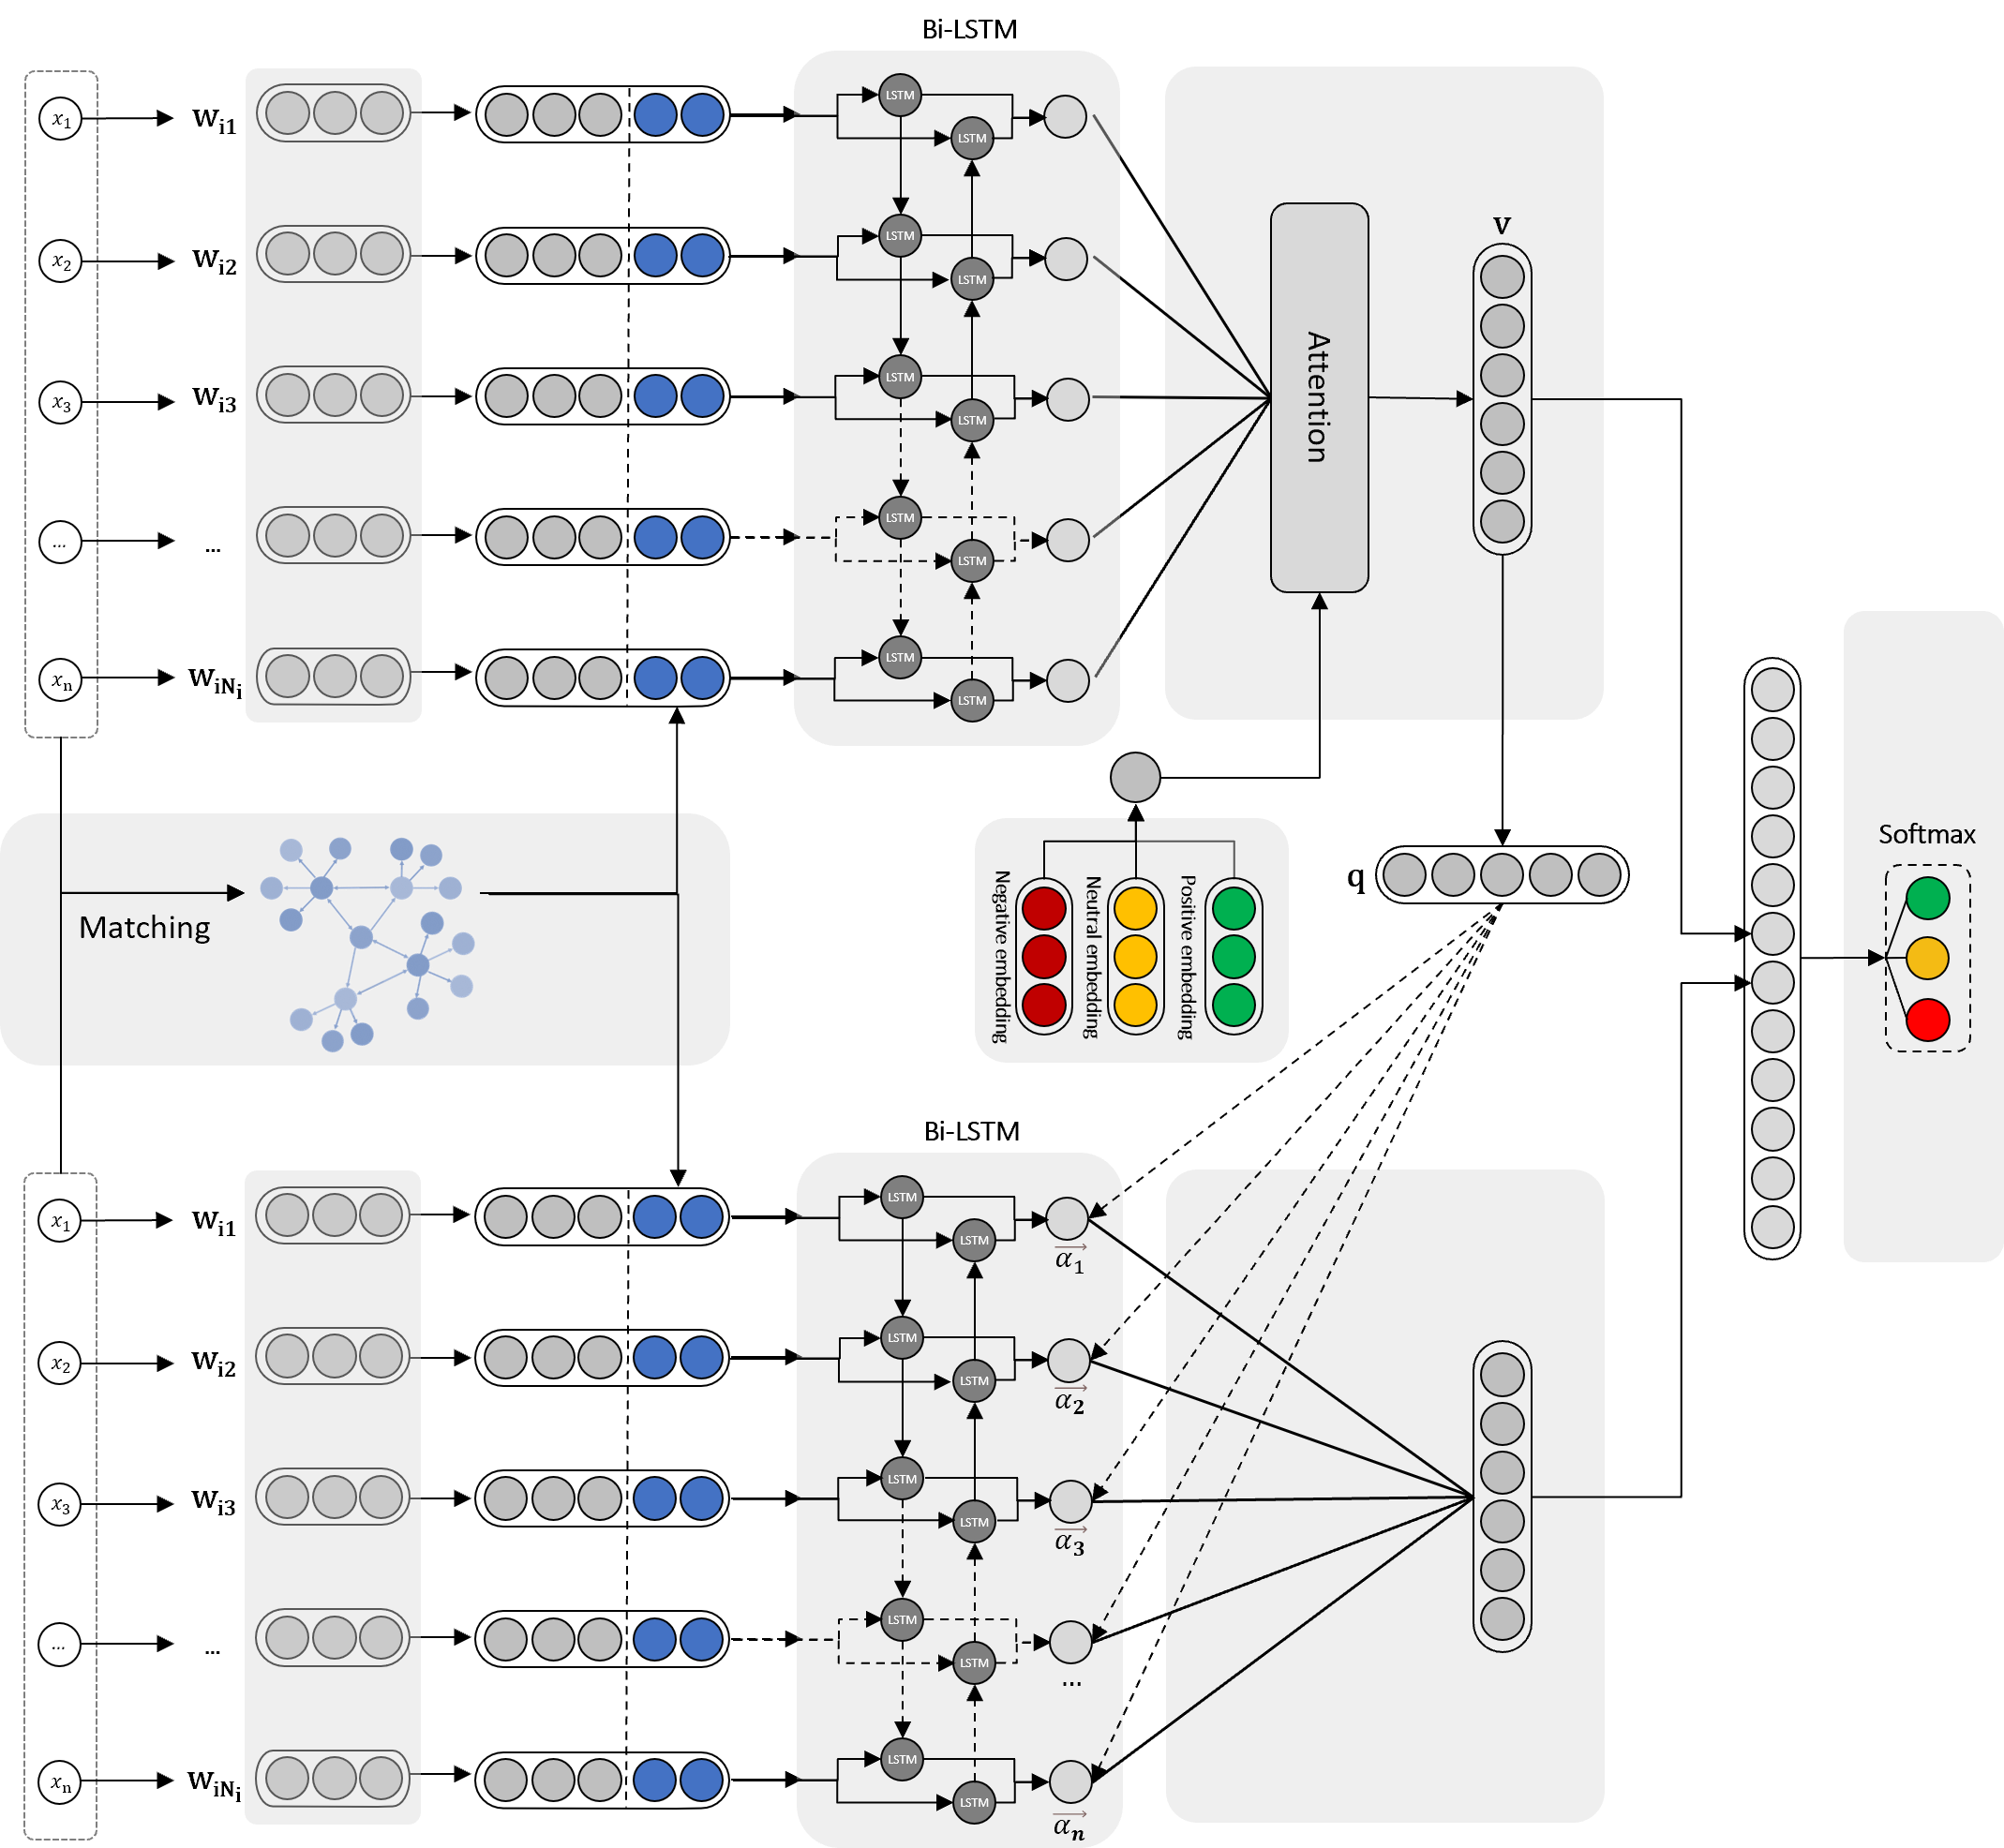
\includegraphics[width=0.8\linewidth]{submissions/knowledge-sentiment-analysis/1.png}
    \caption{Framework of the model}
    \label{fig:framework-of-the-model}
\end{figure}

\paragraph{Input layer}
For the input of the pre-trained model, the implicit sentiment text needs to be encoded first. For the original corpus input, each word or phrase ${x_i}$ in the sentence is hard-coded into the corresponding vector representation by one-hot encoding representation.
The pretrained model uses Transformer as its feature extractor, and also needs to encode the word-by-word position information in the text to obtain the word position representation vector. Finally, the above vector representations are combined and input to the pretrained model to obtain the continuous word embeddings $\vec{w}_{t} \in R^{d_{e}}$ encoded with contextual information, which are used as input information for the next layer.

\paragraph{Adaptive knowledge fusion layer}

In order to better fuse the extracted sentiment knowledge triples with the target implicit sentiment sentence information, a knowledge fusion strategy is needed. For each target implicit sentiment sentence $s$, more than one sentiment knowledge triple may be extracted, i.e., the set of triplets $G=\left\{g_{1}, g_{2}, \ldots, g_{n}\right\}$ can be obtained.
The set of knowledge triplets $G$ extracted from it is regarded as a knowledge graph $G^{i}=\left\{g_{1}^{i}, g_{2}^{i}, \ldots, g_{n}^{i}\right\}$. Using the TranR model \cite{lin2015learning} for each knowledge triple $ g_{j}^{i}=\left(h_{j}, r_{j}, t_{j}\right)$ in $G^{i}$, we obtain the knowledge embedding representation $\boldsymbol{g}_{j}^{i}=\left(\boldsymbol{h}_{j}, \boldsymbol{r}_{j}, \boldsymbol{t}_{j}\right)$. The head entity $h$ is designated as the entity in the target implicit sentiment sentence, and the tail entity $t$ is the entity in the external sentiment knowledge graph.
Using the representations of all head and tail entities learned in the knowledge graph $G^{i}$ in the knowledge subgraphs, their weights are calculated adaptively by the attention mechanism, and the embedded representations of the knowledge subgraphs are learned by this to represent the sentiment cues introduced for the target implicit sentiment sentence, calculated as shown in the Equ.~(\ref{formula_4_1}).
\begin{equation}
    \boldsymbol{G}^{i}=\sum_{j=1}^{n} (\operatorname{softmax}(\boldsymbol{W}_{tv} \boldsymbol{t}_{j}\frac{\boldsymbol{t}_{j}^{T}\boldsymbol{W}_{tk}^{T}\boldsymbol{W}_{h} \boldsymbol{h}_{j}}{\sqrt{d}})+\boldsymbol{W}_{r} \boldsymbol{r}_{j})\label{formula_4_1}
\end{equation}

where $\boldsymbol{W}_{h}, \boldsymbol{W}_{tk},\boldsymbol{W}_{tv}, \boldsymbol{W}_{r} \in \mathbb{R}^{l \times m}$ are the parameter matrices of head entities, tail entities and relations. $\boldsymbol{h}_j, \boldsymbol{t}_j, \boldsymbol{r}_j \in \mathbb{R}^m$.

The knowledge graph embedding representation $\boldsymbol{G}^i$ obtained by learning represents the additional external common knowledge introduced, and if the target sentiment sentence cannot be matched to any sentiment knowledge triplet, $\boldsymbol{G}^i$ is treated as a zero vector.
The word embedding $\boldsymbol{w}_{i}$ obtained in the ``input layer" is fused with $\boldsymbol{G}^i$ to achieve the introduction of external common sense knowledge, and finally the result $\boldsymbol{e}_i=\boldsymbol{ w}_i \oplus \boldsymbol{G}^i$ is input to the next layer.

\paragraph{Multipolar attention layer fusing contextual contexts}

This layer models the fusion of implicit sentiment expressions and contextual information using multipolar attention mechanisms to extend the information in implicit sentiment expressions.

As for the text implicit sentiment classification task, the output of the current moment is not only related to the state before the current moment, but may also related to the state after the current moment.
In this layer, the input of the upper layer network first passes through a bi-directional long and short-term memory network (Bi-LSTM), Bi-LSTM is composed of an LSTM with forward processing sequences and an LSTM with reverse processing sequences, considering both forward and backward sequences, making full use of contextual information and allowing deep feature extraction of the contextual information inside the input sentence.

As mentioned in the literature \cite{wei2020BiLSTM}, the difference between attention weights for specific polarities is an important feature of the Chinese implicit sentiment analysis task.
Therefore, multi-polar attention mechanisms are introduced in this layer to incorporate sentiment polarity labeling information into the implicit sentiment representation. Specifically, polarity-specific queries are introduced by using attention mechanisms with different polarities in order to make the attention mechanism more focused on the differences between different sentiment polarities.The calculation formula are shown in Eq.~(\ref{formula_4_2}), Eq.~(\ref{formula_4_3}), Eq.~(\ref{formula_4_4}).

\begin{equation}
    \boldsymbol{v}^q=\sum_{i=1}^T \alpha_i^q \boldsymbol{t}_i
    \label{formula_4_2}
\end{equation}

\begin{equation}
    \alpha_i^q=\frac{\exp \left(e_i^q\right)}{\sum_{k=1}^T \exp \left(e_k^q\right)}
    \label{formula_4_3}
\end{equation}


\begin{equation}
    e_i^q=\boldsymbol{q} \boldsymbol{W} \boldsymbol{m}_i
    \label{formula_4_4}
\end{equation}

where $ \boldsymbol{v}^q $ represents the embedding representation of sentences under sentiment polarity $q$. $T$ is the length of the target implicit sentiment sentence.$ \alpha_i$ is the normalized weight of the word or character $w_i$ computed from the Bi-LSTM output $ \boldsymbol{t}_i $. $ e^q_i$ is the attention score of $w_i$. The matrix $\boldsymbol{W}$ is then used to query the weight matrix of $q$ and $\boldsymbol{h}_i$ in the bilinear function. $\boldsymbol{q} \in \boldsymbol{Q}=\left\{\boldsymbol{q}_{\text{pos}}, \boldsymbol{q}_{\text{neg}}, \boldsymbol{q}_{\text{neu}}\right\}$ correspond to polarity-specific query embedding representations of positive, negative and neutral sentiment polarity, respectively. The same sentiment dictionary as in the knowledge triad extraction process above is used here to initialize the polarity query embedding representation, which is computed by averaging the embeddings of sentiment words with the same sentiment polarity in the sentiment dictionary, as shown in Eq.~(\ref{formula_4_5}):

\begin{equation}
    \boldsymbol{q}=\frac{1}{N} \sum_{i=1}^N \boldsymbol{w}_i^q
    \label{formula_4_5}
\end{equation}


$\boldsymbol{w}_i^q$ is a pre-trained embedding representation of the word or character $w_i$ whose sentiment polarity belongs to $q$, $q \in Q=\left\{q_{\text {pos }}, q_{\text {neg }}, q_{\text {neu }}\right\}$.

The implicit sentiment sentence representations with weights under the three sentiment polarities are spliced to obtain a new representation of the implicit sentiment expression $\boldsymbol{v}=\boldsymbol{v}^{q_{pos}} \oplus \boldsymbol{v}^{q_{neg}} \oplus \boldsymbol{v}^{q_{neu}}$.


The context representation is considered as a whole, and the implicit sentiment sentence representation $q^c$ transformed by the fully connected layer is used as the query vector to assign weights to each word in $C$ in order to achieve the extraction of key features in the contextual information of the target implicit sentiment expression by the model through the attention mechanism.


\begin{equation}
    \boldsymbol{v^c}=\sum_{i=1}^{T_C} \alpha_j^c \boldsymbol{t}_i
    \label{formula_4_6}
\end{equation}

\begin{equation}
    \alpha_j^c=\frac{\exp \left(e_j^c\right)}{\sum_{k=1}^m \exp \left(e_k^c\right)},
    \label{formula_4_7}
\end{equation}

\begin{equation}
    e_j^c=\boldsymbol{q}^c \boldsymbol{W}^c \boldsymbol{h}_j^c
    \label{formula_4_8}
\end{equation}

\begin{equation}
    \boldsymbol{q}^c=\tanh (\boldsymbol{W} \boldsymbol{v}+\boldsymbol{b})
    \label{formula_4_9}
\end{equation}

Finally, by splicing the implicit sentiment sentence representation $\boldsymbol{v}$ with the contextual representation $\boldsymbol{v^c}$, the implicit sentiment sentence representation $\boldsymbol{v_{out}}$, which incorporates the contextual information, is obtained as the output of this layer, and it is fed into the output layer for the final probability calculation, as shown in Equ.~(\ref{formula_4_10}):
\begin{equation}
    \boldsymbol{v_{out}}=\boldsymbol{v} \oplus \boldsymbol{v^c}
    \label{formula_4_10}
\end{equation}

\paragraph{Output layer}

In the output layer, an implicit sentiment sentence representation $\boldsymbol{v_{out}}$ incorporating contextual information is projected into the sentiment polarity category space using a fully connected network. Then, the scores of each category are normalized to an approximate probability value $\widehat{\boldsymbol{y}}$ by the calculation of the Eq.~(\ref{formula_4_11}).
\begin{equation}
    \widehat{\boldsymbol{y}}=\operatorname{softmax}\left(\boldsymbol{W}_{\text {out }} \boldsymbol{v}^{\mathrm{T}}+\boldsymbol{b}_{\text {out }}\right)
    \label{formula_4_11}
\end{equation}
where $\boldsymbol{W}_{\text{out}}$ and $\boldsymbol{b}_{\text{out}}$ are the weight matrix and bias, respectively.

\section{Experimental Setup}

In this section, we present the details of the datasets used, the methods, and the implementation details of our models.

\subsection{Dataset}

In the field of Chinese implicit sentiment analysis research, the most widely used public dataset is the dataset used in the SMP2019 Chinese Implicit Sentiment Analysis Review (SMP-ECISA 2019) provided by Shanxi University \footnote{https://www.biendata.xyz/competition/ smpecisa2019/data/}.
The corpus of this dataset is collected from social media such as microblogs, travel websites, and product e-commerce, and a large-scale sentiment dictionary is used to filter the collected data, remove sentiment expression sentences with explicit sentiment words, and use the remaining text data as the Chinese implicit sentiment analysis dataset.
The main domains/topics covered in this dataset include but are not limited to: Spring Festival Gala, Haze, LeTV, National Exam, Travel, Dragon Boat Festival, etc. The classification of sentiment labels in the dataset is divided into 3 types: negative, neutral and positive, corresponding to the numerical labels 1, 2 and 0. Tab.~\ref{table:smp-ecisa-2019-dataset}~ shows the detailed statistics of the dataset.

\begin{table}
    \caption{SMP-ECISA 2019 Dataset}
    \label{table:smp-ecisa-2019-dataset}
    \centering
    \scalebox{1.25}{
        \begin{tabular}{cccccc}
            \toprule[1.5pt] %
                           & articles & labeled sentences & neutral & positive & negative \\
            \hline
            Training set   & 12,664   & 1,4774            & 6,989   & 3,828    & 3,957    \\
            Validation set & 4,391    & 5,143             & 2,553   & 1,232    & 1,358    \\
            Test set       & 6,380    & /                 & /       & /        & /        \\
            \hline
            After merging  & 17,055   & 19,917            & 9,542   & 5,060    & 5,315    \\
            \bottomrule[1.5pt]
        \end{tabular}
    }
\end{table}

In order to evaluate and compare existing methods and our method more fairly, we combined the training and validation sets to obtain 17,055 articles with a total of 19,917 labeled data, and re-divided the training set, validation set, and test set in the ratio of 8:1:1, and evaluated them using ten-fold cross-validation, and took the best result as the final result of the model.

\subsection{Evaluation Metrics}

To more reasonably and reliably measure the effectiveness of the method proposed in this paper, the F1 scores of the three emotional polarities and the macro-average F1 scores are calculated as indicators in this paper, as shown in the Eq.~(\ref{formula_4_12}), Eq.~(\ref{formula_4_13}).
\begin{equation}
    F_1i=\frac{2 * P_i * R_i}{P_i+R_i},
    \label{formula_4_12}
\end{equation}

\begin{equation}
    F_1-{\text{macro}}=\frac{1}{N} \sum_{i=1}^N F_1i,
    \label{formula_4_13}
\end{equation}

$i \in\{$ positive, negative, neutral $\}$ is one of the three sentiment polarities, and $P_i$ and $R_i$ are the accuracy and recall corresponding to the sentiment polarity $i$.

\subsection{Implementation Details}

Due to the limitation of the training hardware equipment, we can not train all the corpus at the same time, so the complete training set needs to be divided into many training batches. Based on a careful observation of the dataset, it was found that the corpus data in the dataset varied in length, which led to the internal setting of the model for the input length that may affect the final results of the model. Taking into account the hardware resources of the training environment, we chose 128 as the maximum length of input sentences, with each batch size of 16, and trained 5 epochs in total. For each single item in the BiLSTM, each has a hidden layer unit that needs to be learned by setting different sizes that will change the model's ability to capture features, and we set them all to 128. Additionally, the learning rate was set to 5e-5 and the dropout rate was 0.4.


\subsection{Baseline Methods}

Because of the limited research on the implicit sentiment analysis task of Chinese text, in this section, in addition to selecting some of the latest implicit sentiment analysis models according to the settings in the literature \cite{liao2022dynamic}, some representative models with good results in traditional explicit sentiment analysis tasks\cite{zhang2022incorporating} are selected as baselines for comparison experiments. The baseline experiments are described in detail as follows.

\paragraph{Bi-LSTM+multi-attention} 
The combination of Bi-LSTM combined with attention mechanism has been proven to be an effective model in many tasks related to sentiment analysis. The multi-headed attention mechanism can capture more of the differences between multiple attentions to some extent and enhance the effect even further.

\paragraph{Bi-LSTM+MPOA} 
\label{par:Bi-LSTM+MPOA}
Jiyao et al. \cite{wei2020BiLSTM} proposed an orthogonal multi-attention mechanism and fused it with Bi-LSTM to improve the traditional multi-attention mechanism by using orthogonal attention with specific sentiment polarity.

\paragraph{CMPOA} 
\label{par:CMPOA}
The model that Wang et al. \cite {WangSuGe2022} proposed integrates contextual information into the basic MPOA to compensate for the lack of information in the implicit sentiment sentence itself.


\paragraph{CsHGCN}
\label{par:CsHGCN}
Zuo et al. \cite{zuo2020context} proposed a heterogeneous graph convolutional network model to represent the implicit sentiment sentences. The entire context is treated as a heterogeneous graph at the document level and deep domain features are captured by graph convolution.

\paragraph{Tree-LSTM+KG} 
\label{par:Tree-LSTM+KG}
Syntactic structure information is important for modeling implicit sentiment sentences. The syntactic structure tree of the input sentence is obtained using LTP \cite{che2010ltp}, and then a Tree-LSTM \cite{tai2015improved} based model is constructed to fuse the syntactic structure to the embedding of the sentence.

\section{Results And Analysis}

\begin{table}[!htb]
    \caption{Performance of Chinese implicit sentiment analysis}
    \label{table:6_1}
    \centering
    \begin{tabular}{llllll}
        \toprule[1.5pt] 
        \textbf{Methods}              & \textbf{PLM} & \textbf{$F_{neu}$} & \textbf{$F_{pos}$} & \textbf{$F_{neg}$} & \textbf{$F_1$-macro} \\
        \hline
        SDT-CNN                       &              & 0.735              & 0.701              & 0.697              & 0.711                \\
        TextCNN                       &              & 0.734              & 0.724              & 0.712              & 0.723                \\
        CsHGCN                        &              & 0.848              & 0.670              & 0.775              & 0.764                \\
        BiLSTM + Att                  &              & 0.800              & 0.630              & 0.747              & 0.726                \\
        BiLSTM + Mult-Att             &              & 0.810              & 0.634              & 0.749              & 0.730                \\
        \multirow{3}*{CMPOA}          & random       & 0.800              & 0.568              & 0.702              & 0.690                \\
        ~                             & BERT         & 0.784              & 0.585              & 0.712              & 0.694                \\
        ~                             & ERNIE        & 0.816              & 0.662              & 0.761              & 0.746                \\
        \multirow{3}*{TreeLSTM+KG}    & random       & 0.750              & 0.560              & 0.692              & 0.667                \\
        ~                             & BERT         & 0.764              & 0.581              & 0.725              & 0.690                \\
        ~                             & ERNIE        & 0.805              & 0.650              & 0.779              & 0.745                \\
        \multirow{3}*{BiLSTM+MPOA}    & random       & 0.764              & 0.569              & 0.691              & 0.675                \\
        ~                             & BERT         & 0.808              & 0.684              & 0.669              & 0.720                \\
        ~                             & ERNIE        & 0.834              & 0.690              & 0.791              & 0.775                \\
        \multirow{3}*{LSTM+Att+KG}    & random       & 0.759              & 0.558              & 0.690              & 0.669                \\
        ~                             & BERT         & 0.771              & 0.593              & 0.732              & 0.699                \\
        ~                             & ERNIE        & 0.802              & 0.643              & 0.781              & 0.742                \\
        \multirow{3}*{BiLSTM+MPOA+KG} & random       & 0.773              & 0.554              & 0.692              & 0.673                \\
        ~                             & BERT         & 0.792              & 0.593              & 0.710              & 0.699                \\
        ~                             & ERNIE        & 0.819              & 0.655              & 0.749              & 0.741                \\
        \hline
        \multirow{3}*{Ours}           & random       & 0.789              & 0.571              & 0.702              & 0.687                \\
        ~                             & BERT         & 0.803              & 0.582              & 0.716              & 0.699                \\
        ~                             & ERNIE        & \textbf{0.849}     & \textbf{0.690}     & \textbf{0.799}     & \textbf{0.778}       \\
        \bottomrule[1.5pt]
    \end{tabular}
\end{table}

\subsection{Comparison with Baselines}

Experiment results are reported in Table.~\ref{table:6_1}, and by observing and analyzing the results it can be found that:

From the overall view of each metric, the method proposed in this paper has the best results on all metrics, indicating that our method can effectively improve the effectiveness of the implicit sentiment analysis task. Specifically, in our experiments, we compare the model proposed in this paper with models that have been effective in traditional explicit sentiment analysis tasks and with existing implicit sentiment analysis models, and our model obtained the best results.

Our model has a large improvement in the implicit sentiment analysis task compared to the traditional explicit sentiment analysis model, which indicates that the traditional explicit sentiment analysis approach has some shortcomings in the implicit sentiment analysis task.
Further, from the results of the model without the introduction of common sense knowledge information, it can be found that the introduction of additional external common sense knowledge has a 4\% improvement in the $F_1-macro$ metric for the implicit sentiment analysis task, which indicates that the introduction of the triplet  of common sense knowledge can provide critical sentiment information and can effectively compensate for the lack of information caused by the absence of explicit sentiment words.
On the other hand, the result analysis of the model without introducing contextual information illustrates that for the target implicit sentiment expression, fusion with contextual information can extend the sentiment semantic information of implicit sentiment sentences from another aspect to enhance the implicit sentiment analysis.
The above results and analysis show that effective extension of the implicit sentiment sentence representation can be achieved by fusing the common sense knowledge information provided by the external knowledge base with the contextual representation and the semantic information of the sentiment expression itself.

Meanwhile, the common sense knowledge fusion method proposed in this paper can effectively improve the interpretability of the model. Traditional methods, such as BiLSTM+MPOA, usually interpret the prediction results based on the attention weights of words in the sentence only. However, in implicit sentiment analysis tasks, words with higher attention weights are usually also neutral or objective words. The reason for the model prediction can be demonstrated by introducing external common sense knowledge. Take the sentence ``I got a good grade in this exam" as an example, the positive sentiment predicted by the model can be explained by the sentiment triple $(getting\ a\ good\ grade, causes, praise)$, which makes the prediction more intuitive and convincing.
In summary, the experimental results show that the method in this paper has improved the performance of Chinese implicit sentiment analysis and has shown the ability to interpret the results to a certain extent.

\begin{table}[!htb]
    \caption{Performance of Chinese implicit sentiment analysis The ablations of different components are reported separately in this table, where the model without additional explicit introduction of external common sense knowledge is denoted as ‘-KG’, ‘-MPA’ indicates that no multipolar orthogonal attention mechanism is used in the process of sentiment representation and knowledge incorporation, and ‘-Context’ indicates that no additional contextual information of additional sentiment representation is introduced.}

    \label{table:6_2}
    \centering
    \scalebox{1.2}{
        \begin{tabular}{lllll}
            \toprule[1.5pt] 
            \textbf{Methods} & \textbf{$F_{neu}$} & \textbf{$F_{pos}$} & \textbf{$F_{neg}$} & \textbf{$F_1$-macro} \\
            \hline
            Ours             & \textbf{0.849}     & \textbf{0.690}     & \textbf{0.799}     & \textbf{0.778}       \\
            -KG              & 0.816              & 0.662              & 0.761              & 0.746                \\
            -MPA             & 0.827              & 0.674              & 0.782              & 0.761                \\
            -Context         & 0.819              & 0.655              & 0.749              & 0.741                \\
            \bottomrule[1.5pt]
        \end{tabular}
    }
\end{table}

\subsection{Ablation Study}

Tab.~\ref{table:6_2} shows the results of the metrics after removing each component from our model separately. The results of the three ablation experiments show that each component of the proposed method in this paper contributes to the model to some extent.

Specifically, removing the introduction of external knowledge has the greatest impact on the model's effectivenes; without the use of external common sense knowledge (`-KG'), we observe a more dramatic decrease in performance compared to all other components, with a decrease of nearly 4.1\% in $F_1-macro$, demonstrating the effectiveness and importance of introducing additional common sense knowledge for the implicit sentiment analysis task, which can effectively complement the implicit sentiment expression sentiment cues that are missing due to the absence of explicit sentiment vocabulary.
The next most effective effect of removing the introduction of contextual information on the model, with an overall performance decrease of 3.4\% when focusing only on the semantic information of the implicit sentiment expression itself (-Context'), which indicates that contextual information is also more significant for understanding the implicit sentiment expression and can be used when the implicit sentiment expression. This indicates that contextual information is also important for understanding implicit sentiment expressions, and can offer effective sentiment semantic information when the implicit sentiment expressions cannot provide sufficient sentiment features by their own information.
Finally, the multi-polar attention mechanism has the least effect on the model, and the addition of MPA mechanism improves the model by about 2.1\%, which also indicates that the  MPA mechanism is somewhat helpful, but not as effective as the above two components.

In summary, the various components used in the model proposed in this paper are all instrumental for the implicit sentiment analysis task.

\section{Conclusion}

In this paper, we propose a sentiment analysis method incorporating contextual information and external common sense knowledge for implicit sentiment analysis.
We first propose a retrieval method to extract valid sentiment triads from a knowledge base and build an adaptive fusion of external common sense knowledge embedding layers to extend the semantic information of implicit sentiment expressions.
Multi-polar attention mechanism is then used to learn embedding representations for implicit sentiment expressions, and an attention layer that incorporates context is introduced to mine and combine valid information in the context.
Finally, the common sense knowledge information provided by the external knowledge base is fused with the contextual representation and the semantic information of the sentiment expression itself to achieve an effective extension of the implicit sentiment sentence representation and to perform sentiment label prediction.
Experimental results on the SMP2019-ECISA dataset show that the method outperforms existing state-of-the-art methods and can fully exploit contextual information and external common sense knowledge to effectively improve the analysis of implicit sentiment expressions.


\section{Acknowledgments}
%The authors would like to thank the anonymous reviewers for insightful comments and helpful suggestions.
This work was supported by National Natural Science Foundation of China (No.62176185)

%\bibliographystyle{plain}
%\bibliography{submissions/knowledge-sentiment-analysis/main}

\begin{thebibliography}{10}

\bibitem{balahur2011detecting}
Alexandra Balahur, Jes{\'u}s~M Hermida, and Andr{\'e}s Montoyo.
\newblock Detecting implicit expressions of sentiment in text based on
  commonsense knowledge.
\newblock In {\em Proceedings of the 2nd Workshop on Computational Approaches
  to Subjectivity and Sentiment Analysis (WASSA 2.011)}, pages 53--60, 2011.

\bibitem{balahur2012detecting}
Alexandra Balahur, Jes{\'u}s~M Hermida, and Andr{\'e}s Montoyo.
\newblock Detecting implicit expressions of emotion in text: A comparative
  analysis.
\newblock {\em Decision support systems}, 53(4):742--753, 2012.

\bibitem{bordes2013translating}
Antoine Bordes, Nicolas Usunier, Alberto Garcia-Duran, Jason Weston, and Oksana
  Yakhnenko.
\newblock Translating embeddings for modeling multi-relational data.
\newblock {\em Advances in neural information processing systems}, 26, 2013.

\bibitem{che2010ltp}
Wanxiang Che, Zhenghua Li, and Ting Liu.
\newblock Ltp: A chinese language technology platform.
\newblock In {\em Coling 2010: Demonstrations}, pages 13--16, 2010.

\bibitem{chen2016implicit}
Huan-Yuan Chen and Hsin-Hsi Chen.
\newblock Implicit polarity and implicit aspect recognition in opinion mining.
\newblock In {\em Proceedings of the 54th Annual Meeting of the Association for
  Computational Linguistics (Volume 2: Short Papers)}, pages 20--25, 2016.

\bibitem{ChenQiuChang2022}
Qiuchang CHEN, Hui ZHAO, Enguang ZUO, ZHAO Yuxia, and Wenyu WEI.
\newblock Implicit sentiment analysis based on context aware tree recurrent
  neutral network.
\newblock {\em Computer Engineering and Applications}, 58(07):167--175.

\bibitem{erik2017sentiment}
Cambria Erik, Poria Soujanya, Gelbukh Alexander, and Thelwall Mike.
\newblock Sentiment analysis is a big suitcase.
\newblock {\em IEEE Intelligent Systems}, 32(6):74--80, 2017.

\bibitem{jian2016constitution}
Liao Jian, Li~Yang, and Wang Suge.
\newblock The constitution of a fine-grained opinion annotated corpus on weibo.
\newblock In {\em Chinese Computational Linguistics and Natural Language
  Processing Based on Naturally Annotated Big Data}, pages 227--240. Springer,
  2016.

\bibitem{li2022c3kg}
Dawei Li, Yanran Li, Jiayi Zhang, Ke~Li, Chen Wei, Jianwei Cui, and Bin Wang.
\newblock C3kg: A chinese commonsense conversation knowledge graph.
\newblock {\em arXiv preprint arXiv:2204.02549}, 2022.

\bibitem{LiaoJian2018}
Jian Liao.
\newblock {\em Research on Fact-implied Implicit Sentiment Analysis Based on
  Representation Learning}.
\newblock PhD thesis, Shanxi University, 2018.

\bibitem{liao2022dynamic}
Jian Liao, Min Wang, Xin Chen, Suge Wang, and Kai Zhang.
\newblock Dynamic commonsense knowledge fused method for chinese implicit
  sentiment analysis.
\newblock {\em Information Processing \& Management}, 59(3):102934, 2022.

\bibitem{liao2019identification}
Jian Liao, Suge Wang, and Deyu Li.
\newblock Identification of fact-implied implicit sentiment based on
  multi-level semantic fused representation.
\newblock {\em Knowledge-Based Systems}, 165:197--207, 2019.

\bibitem{liao2017freerl}
Jian Liao, Suge Wang, Deyu Li, and Xiaoli Li.
\newblock Freerl: Fusion relation embedded representation learning framework
  for aspect extraction.
\newblock {\em Knowledge-Based Systems}, 135:9--17, 2017.

\bibitem{lin2015learning}
Yankai Lin, Zhiyuan Liu, Maosong Sun, Yang Liu, and Xuan Zhu.
\newblock Learning entity and relation embeddings for knowledge graph
  completion.
\newblock In {\em Twenty-ninth AAAI conference on artificial intelligence},
  2015.

\bibitem{liu2020sentiment}
Bing Liu.
\newblock {\em Sentiment analysis: Mining opinions, sentiments, and emotions}.
\newblock Cambridge university press, 2020.

\bibitem{mason2004cormet}
Zachary~J Mason.
\newblock Cormet: a computational, corpus-based conventional metaphor
  extraction system.
\newblock {\em Computational linguistics}, 30(1):23--44, 2004.

\bibitem{mehndiratta2017detection}
Pulkit Mehndiratta, Shelly Sachdeva, and Devpriya Soni.
\newblock Detection of sarcasm in text data using deep convolutional neural
  networks.
\newblock {\em Scalable Computing: Practice and Experience}, 18(3):219--228,
  2017.

\bibitem{PanDongXing2020}
Donghang PAN, Jingling YUAN, Lin Li, and Deming SHENG.
\newblock A chinese implicit sentiment classification model combining
  contextual features.
\newblock {\em Computer Engineering \& Science}, 42(2):10, 2020.

\bibitem{qian2018hierarchical}
Jing Qian, Mai ElSherief, Elizabeth Belding, and William~Yang Wang.
\newblock Hierarchical cvae for fine-grained hate speech classification.
\newblock {\em arXiv preprint arXiv:1809.00088}, 2018.

\bibitem{samuel2022direct}
David Samuel, Jeremy Barnes, Robin Kurtz, Stephan Oepen, Lilja {\O}vrelid, and
  Erik Velldal.
\newblock Direct parsing to sentiment graphs.
\newblock {\em arXiv preprint arXiv:2203.13209}, 2022.

\bibitem{sap2019atomic}
Maarten Sap, Ronan Le~Bras, Emily Allaway, Chandra Bhagavatula, Nicholas
  Lourie, Hannah Rashkin, Brendan Roof, Noah~A Smith, and Yejin Choi.
\newblock Atomic: An atlas of machine commonsense for if-then reasoning.
\newblock In {\em Proceedings of the AAAI conference on artificial
  intelligence}, volume~33, pages 3027--3035, 2019.

\bibitem{shutova2017multilingual}
Ekaterina Shutova, Lin Sun, Elkin~Dar{\'\i}o Guti{\'e}rrez, Patricia
  Lichtenstein, and Srini Narayanan.
\newblock Multilingual metaphor processing: Experiments with semi-supervised
  and unsupervised learning.
\newblock {\em Computational Linguistics}, 43(1):71--123, 2017.

\bibitem{shutova2013statistical}
Ekaterina Shutova, Simone Teufel, and Anna Korhonen.
\newblock Statistical metaphor processing.
\newblock {\em Computational Linguistics}, 39(2):301--353, 2013.

\bibitem{tai2015improved}
Kai~Sheng Tai, Richard Socher, and Christopher~D Manning.
\newblock Improved semantic representations from tree-structured long
  short-term memory networks.
\newblock {\em arXiv preprint arXiv:1503.00075}, 2015.

\bibitem{J2008LakoffGeorge}
J.~P. Thorne.
\newblock Lakoffgeorge and johnsonmark, metaphors we live by. chicago and
  london: The university of chicago press, 1980. pp. xiii + 242.
  bolingerdwight, language the loaded weapon: the use \& abuse of language
  today. london and new york: Longman, 1980. pp. ix + 214.
\newblock {\em Journal of Linguistics}, 19(1):245--248, 2008.

\bibitem{tong2013can}
Eddie~MW Tong, Deborah~H Tan, and Yan~Lin Tan.
\newblock Can implicit appraisal concepts produce emotion-specific effects? a
  focus on unfairness and anger.
\newblock {\em Consciousness and cognition}, 22(2):449--460, 2013.

\bibitem{vaswani2017attention}
Ashish Vaswani, Noam Shazeer, Niki Parmar, Jakob Uszkoreit, Llion Jones,
  Aidan~N Gomez, {\L}ukasz Kaiser, and Illia Polosukhin.
\newblock Attention is all you need.
\newblock {\em Advances in neural information processing systems}, 30, 2017.

\bibitem{wang2020chinese}
Hongbin Wang, Minghui Hou, Fan Li, and Yafei Zhang.
\newblock Chinese implicit sentiment analysis based on hierarchical knowledge
  enhancement and multi-pooling.
\newblock {\em IEEE Access}, 8:126051--126065, 2020.

\bibitem{WangSuGe2022}
Suge WANG, Min WANG, Jian LIAO, and Xin CHEN.
\newblock An implicit sentiment sentence identification method base on context
  information.
\newblock {\em Journal of Shanxi University(Natural Science Edition)},
  45(02):380--386.

\bibitem{wei2020BiLSTM}
Jiyao Wei, Jian Liao, Zhenfei Yang, Suge Wang, and Qiang Zhao.
\newblock Bi-lstm with multi-polarity orthogonal attention for implicit
  sentiment analysis.
\newblock {\em Neurocomputing}, 383:165--173, 2020.

\bibitem{YangShanLiang2021}
Shanliang YANG and CHANG Zheng.
\newblock Chinese implicit sentiment analysis based on graph attention neural
  network.
\newblock {\em Computer Engineering and Applications}, 57(24):161--167.

\bibitem{zhang2022incorporating}
Kai Zhang, Kun Zhang, Mengdi Zhang, Hongke Zhao, Qi~Liu, Wei Wu, and Enhong
  Chen.
\newblock Incorporating dynamic semantics into pre-trained language model for
  aspect-based sentiment analysis.
\newblock {\em arXiv preprint arXiv:2203.16369}, 2022.

\bibitem{zhang2011identifying}
Lei Zhang and Bing Liu.
\newblock Identifying noun product features that imply opinions.
\newblock In {\em Proceedings of the 49th annual meeting of the Association for
  Computational Linguistics: human language technologies}, pages 575--580,
  2011.

\bibitem{ZhaoRongMei2020}
Rongmei ZHAO, Xi~XIONG, Shenggen JU, Zhongzhi LI, and Chuan XIE.
\newblock Implicit sentiment analysis for chinese texts based on a hybrid
  neural network.
\newblock {\em Journal of Sichuan University(Natural Science Edition)},
  57(2):264--270, 2020.

\bibitem{zhao2012collocation}
Yanyan Zhao, Bing Qin, and Ting Liu.
\newblock Collocation polarity disambiguation using web-based pseudo contexts.
\newblock In {\em Proceedings of the 2012 Joint Conference on Empirical Methods
  in Natural Language Processing and Computational Natural Language Learning},
  pages 160--170, 2012.

\bibitem{zuo2020context}
Enguang Zuo, Hui Zhao, Bo~Chen, and Qiuchang Chen.
\newblock Context-specific heterogeneous graph convolutional network for
  implicit sentiment analysis.
\newblock {\em IEEE Access}, 8:37967--37975, 2020.

\end{thebibliography}
\end{document}

